\documentclass[tikz,border=6pt]{standalone}
\usepackage{pgfplots}
\pgfplotsset{compat=1.18}
\begin{document}
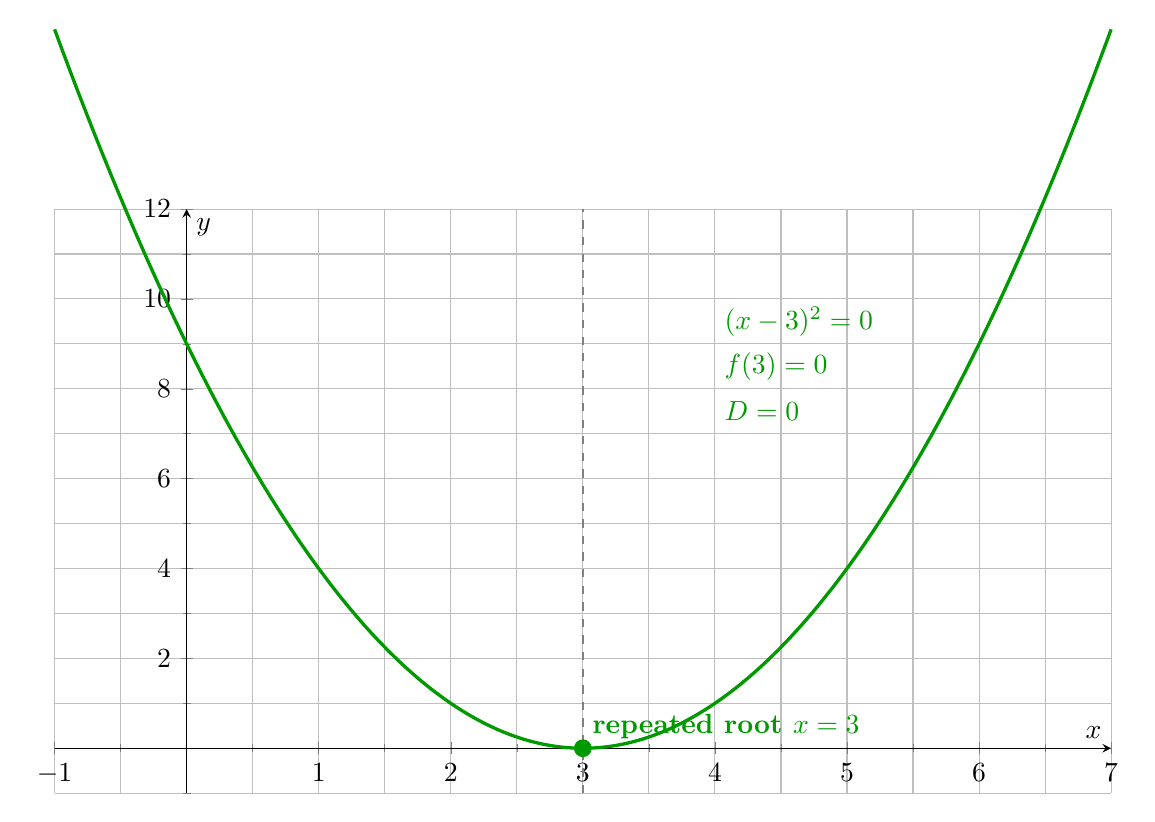
\begin{tikzpicture}
\begin{axis}[
  width=15cm,height=9cm,
  xmin=-1,xmax=7,ymin=-1,ymax=12,
  axis lines=middle,
  xlabel={$x$},ylabel={$y$},
  grid=both,minor tick num=1,
  samples=240,clip=false
]
\addplot[green!60!black,very thick,domain=-1:7]{x^2-6*x+9};
\addplot[gray,dashed,thick] coordinates {(3,-1) (3,12)};
\addplot[green!60!black,only marks,mark=*,mark size=3pt] coordinates {(3,0)};
\node[green!60!black,font=\bfseries,anchor=south west] at (axis cs:3,0) {repeated root $x=3$};
\node[green!60!black,font=\bfseries,anchor=west] at (axis cs:4.0,9.5) {$(x-3)^2=0$};
\node[green!60!black,font=\bfseries,anchor=west] at (axis cs:4.0,8.5) {$f(3)=0$};
\node[green!60!black,font=\bfseries,anchor=west] at (axis cs:4.0,7.5) {$D=0$};
\end{axis}
\end{tikzpicture}
\end{document}
